Nhóm quyết định chọn quy trình đổi vé máy bay để làm case study cũng như kiểm chứng kết quả tính toán được sử dụng cơ sở lý thuyết được trình bày ở trên, so với kết quả thực tế của hệ thống.

\subsection{Thu thập dữ liệu khảo sát}

\begin{center}
    \begin{table}[H]
        \centering
        \def\arraystretch{1.5}%
        \begin{tabular}{|C{1cm}|p{13cm}|}
        \hline
        \textbf{STT} & \multicolumn{1}{c|}{\textbf{Câu hỏi}} \\ \hline
        1 & Do you use any services or products provided by this process? \\ \hline
        2 & What is your role in this process? \\ \hline
        3 & To what extent do you agree with this statement: "It is easy to handle exceptions in your process". \\ \hline
        4 & To what extent do you agree with this statement: "It is easy to execute your process." \\ \hline
        5 & How frequently do exceptions happen in practice? \\ \hline
        6 & Which handled exceptions do you think the way to handle them needs optimizing? Can you suggest some solutions to those? \\ \hline
        7 & Can you suggest any exceptions that need handling and the way to handle them? \\ \hline
        8 & How satisfied are you with the way exceptions are handled in your process? \\ \hline
        9 & How satisfied are you with the amount of time you have to spend on this process? \\ \hline
        10 & A flexible process means it has variations for different conditions. How satisfied are you with those variations of the process? \\ \hline
        11 & How satisfied are you with the cost of products or services of this process? \\ \hline
        12 & How satisfied are you with the products or services provided by this process? \\ \hline
        13 & How satisfied are you with the total time you have to spend on waiting for the output of this process? \\ \hline
        14 & Do you encounter any problems while using products or services provided by this process? \\ \hline
        15 & How likely is it that you would recommend this process to others? \\ \hline
        \end{tabular}
        \caption{Bảng câu hỏi khảo sát}
    \end{table}
\end{center}

Đây là tất cả câu hỏi mẫu có sẵn trong bảng khảo sát, được thiết kế để có thể được sử dụng ở nhiều loại quy trình tương ứng với những nghiệp vụ khác nhau. 
Ở đây, chúng tôi sẽ kiểm chứng kết quả đánh giá của hệ thống, so với kết quả chúng tôi tự tính toán được bằng tay. Trong trường hợp này, 
chúng tôi sẽ lấy dữ liệu từ 10 người dùng khác nhau. Và để kiểm chứng kết quả, chúng tôi sẽ chỉ lấy dữ liệu ở những loại câu hỏi được sử dụng để 
tính giá trị các độ đo cũng như kết quả cuối cùng của bài khảo sát. Cụ thể, chúng tôi sẽ quan tâm dữ liệu ở các câu:
\begin{enumerate}
    \item Loại câu hỏi rẽ nhánh: câu 1
    \item Loại câu hỏi CES: câu 3, câu 4
    \item Loại câu hỏi CSAT: câu 8, câu 9, câu 10, câu 11, câu 12, câu 13
    \item Loại câu hỏi NPS: 15
\end{enumerate}

Ở đây, để dễ dàng cho việc tính toán bằng tay, chúng tôi thiết lập trọng số cho mỗi câu hỏi trong mỗi nhóm độ đo là như nhau. Bên dưới là dữ liệu thu thập được từ bảng khảo sát:

\begin{table}[H]
    \def\arraystretch{1.5}%
    \centering
    \resizebox{\textwidth}{!}{%
        \begin{tabular}{|C{1cm}|p{1cm}|C{1cm}|C{1cm}|C{1cm}|C{1cm}|C{1.2cm}|C{1.2cm}|C{1.2cm}|C{1.2cm}|C{1.2cm}|}
            \hline
                \textbf{Người dùng} & 
                \textbf{Nhóm} & 
                \textbf{Câu 3} & 
                \textbf{Câu 4} & 
                \textbf{Câu 8} & 
                \textbf{Câu 9} & 
                \textbf{Câu 10} &
                \textbf{Câu 11} &
                \textbf{Câu 12} &
                \textbf{Câu 13} &
                \textbf{Câu 15} 
            \\ \hline
                \textbf{1} &
                user &
                6 &
                5 &
                7 &
                4 &
                3 &
                &
                &
                &
                8 
            \\ \hline
                \textbf{2} &
                guest &
                &
                &
                &
                &
                &
                7 &
                6 &
                4 &
                9 
            \\ \hline
                \textbf{3} &
                guest &
                &
                &
                &
                &
                &
                6 &
                7 &
                5 &
                6 
            \\ \hline
                \textbf{4} &
                user &
                7 &
                4 &
                2 &
                4 &
                5 &
                &
                &
                &
                5 
            \\ \hline
                \textbf{5} &
                guest &
                &
                &
                &
                &
                &
                5 &
                7 &
                7 &
                10 
            \\ \hline
                \textbf{6} &
                user &
                7 &
                7 &
                5 &
                6 &
                4 &
                &
                &
                &
                9 
            \\ \hline
                \textbf{7} &
                user &
                6 &
                6 &
                7 &
                2 &
                7 &
                &
                &
                &
                8 
            \\ \hline
                \textbf{8} &
                user &
                5 &
                4 &
                5 &
                3 &
                5 &
                &
                &
                &
                7 
            \\ \hline
                \textbf{9} &
                user &
                6 &
                7 &
                6 &
                7 &
                4 &
                &
                &
                &
                9 
            \\ \hline
                \textbf{10} &
                guest &
                &
                &
                &
                &
                &
                7 &
                5 &
                6 &
                8 
            \\ \hline
        \end{tabular}
    }
    \caption{Bảng chi tiết lựa chọn của người dùng cho mỗi câu hỏi}
\end{table}

\subsection{Kiểm chứng dữ liệu khảo sát}

Như vậy, theo như lý thuyết về các độ đo trong bảng khảo sát, ta có thể tính toán được các biến số cần để tinh ra giá trị cuối cùng của mỗi độ đo.
Nhắc lại, số người đồng ý với câu hỏi (CES) hay số người hài lòng (CSAT) được tính khi người đó cho số điểm nằm trong khoảng [5, 7] cho câu hỏi CES 
hoặc CSAT. Số người thuộc nhóm Promoters khi họ cho điểm cho câu hỏi NPS thuộc tập giá trị {9, 10} và thuộc nhóm Detractors khi họ cho điểm cho câu hỏi 
NPS thuộc tập giá trị \{0, 6\}.
\begin{table}[H]
    \def\arraystretch{1}%
    \centering
    \resizebox{\textwidth}{!}{%
        \begin{tabular}{|C{1cm}|C{1cm}|C{2.5cm}|C{2.75cm}|C{2.75cm}|C{2.75cm}|C{1cm}|}
        \hline
        \textbf{Câu hỏi} &
        \textbf{Phân loại} &
        \textbf{Số người đồng ý với câu hỏi (CES)} &
        \textbf{Số người hài lòng (CSAT)} &
        \textbf{Số người thuộc nhóm Promoters} &
        \textbf{Số người thuộc nhóm Detractors} &
        \textbf{Điểm}
        \\ \hline
            \textbf{3} &
            CES &
            \multicolumn{1}{c|}{6} &
            \multicolumn{1}{l|}{} &
            &
            &
            0.6 
        \\ \hline
            \textbf{4} &
            CES &
            \multicolumn{1}{c|}{4} &
            \multicolumn{1}{l|}{} &
            &
            &
            0.4 
        \\ \hline
            \textbf{8} &
            CSAT &
            &
            5 &
            &
            &
            0.5 
        \\ \hline
            \textbf{9} &
            CSAT &
            &
            2 &
            &
            &
            0.2 
        \\ \hline
            \textbf{10} &
            CSAT &
            &
            3 &
            &
            &
            0.3 
        \\ \hline
            \textbf{11} &
            CSAT &
            &
            4 &
            &
            &
            0.4 
        \\ \hline
            \textbf{12} &
            CSAT &
            &
            4 &
            &
            &
            0.4 
        \\ \hline
            \textbf{13} &
            CSAT &
            &
            3 &
            &
            &
            0.3 
        \\ \hline
            \textbf{15} &
            NPS &
            &
            \multicolumn{1}{l|}{} &
            \multicolumn{1}{c|}{4} &
            \multicolumn{1}{c|}{2} &
            0.2 
        \\ \hline
        \end{tabular}
    }
    \caption{Bảng kết quả tính toán mỗi câu hỏi}
\end{table}
Mỗi câu hỏi đều có trọng số như nhau, và mỗi độ đo đều có trọng số như nhau trong bảng khảo sát, như vậy ta có điểm số của từng độ đo và của bài khảo sát: CES = 0.833, CSAT = 0.736, NPS = 0.2.
% \begin{table}[H]
%     \centering
%     \resizebox{\textwidth}{!}{%
%     \begin{tabular}{|C{2.2cm}|C{2.2cm}|C{2.2cm}|C{2.2cm}|C{2.2cm}|C{2.2cm}|}
%     \hline
%     \textbf{Độ đo} & \textbf{Điểm} & \textbf{Độ đo} & \textbf{Điểm} & \textbf{Độ đo} & \textbf{Điểm} \\ \hline
%     CES            & 0.833           & CSAT           & 0.736          & NPS            & 0.2           \\ \hline
%     \end{tabular}%
%     }
%     \caption{Bảng kết quả tổng hợp của khảo sát}
% \end{table}
Từ đó, ta tính được điểm tổng của bài khảo sát là 0.59.
Đối chiếu với kết quả tính được từ hệ thống như sau:
\begin{center}
    \begin{figure}[H]
        \centering
        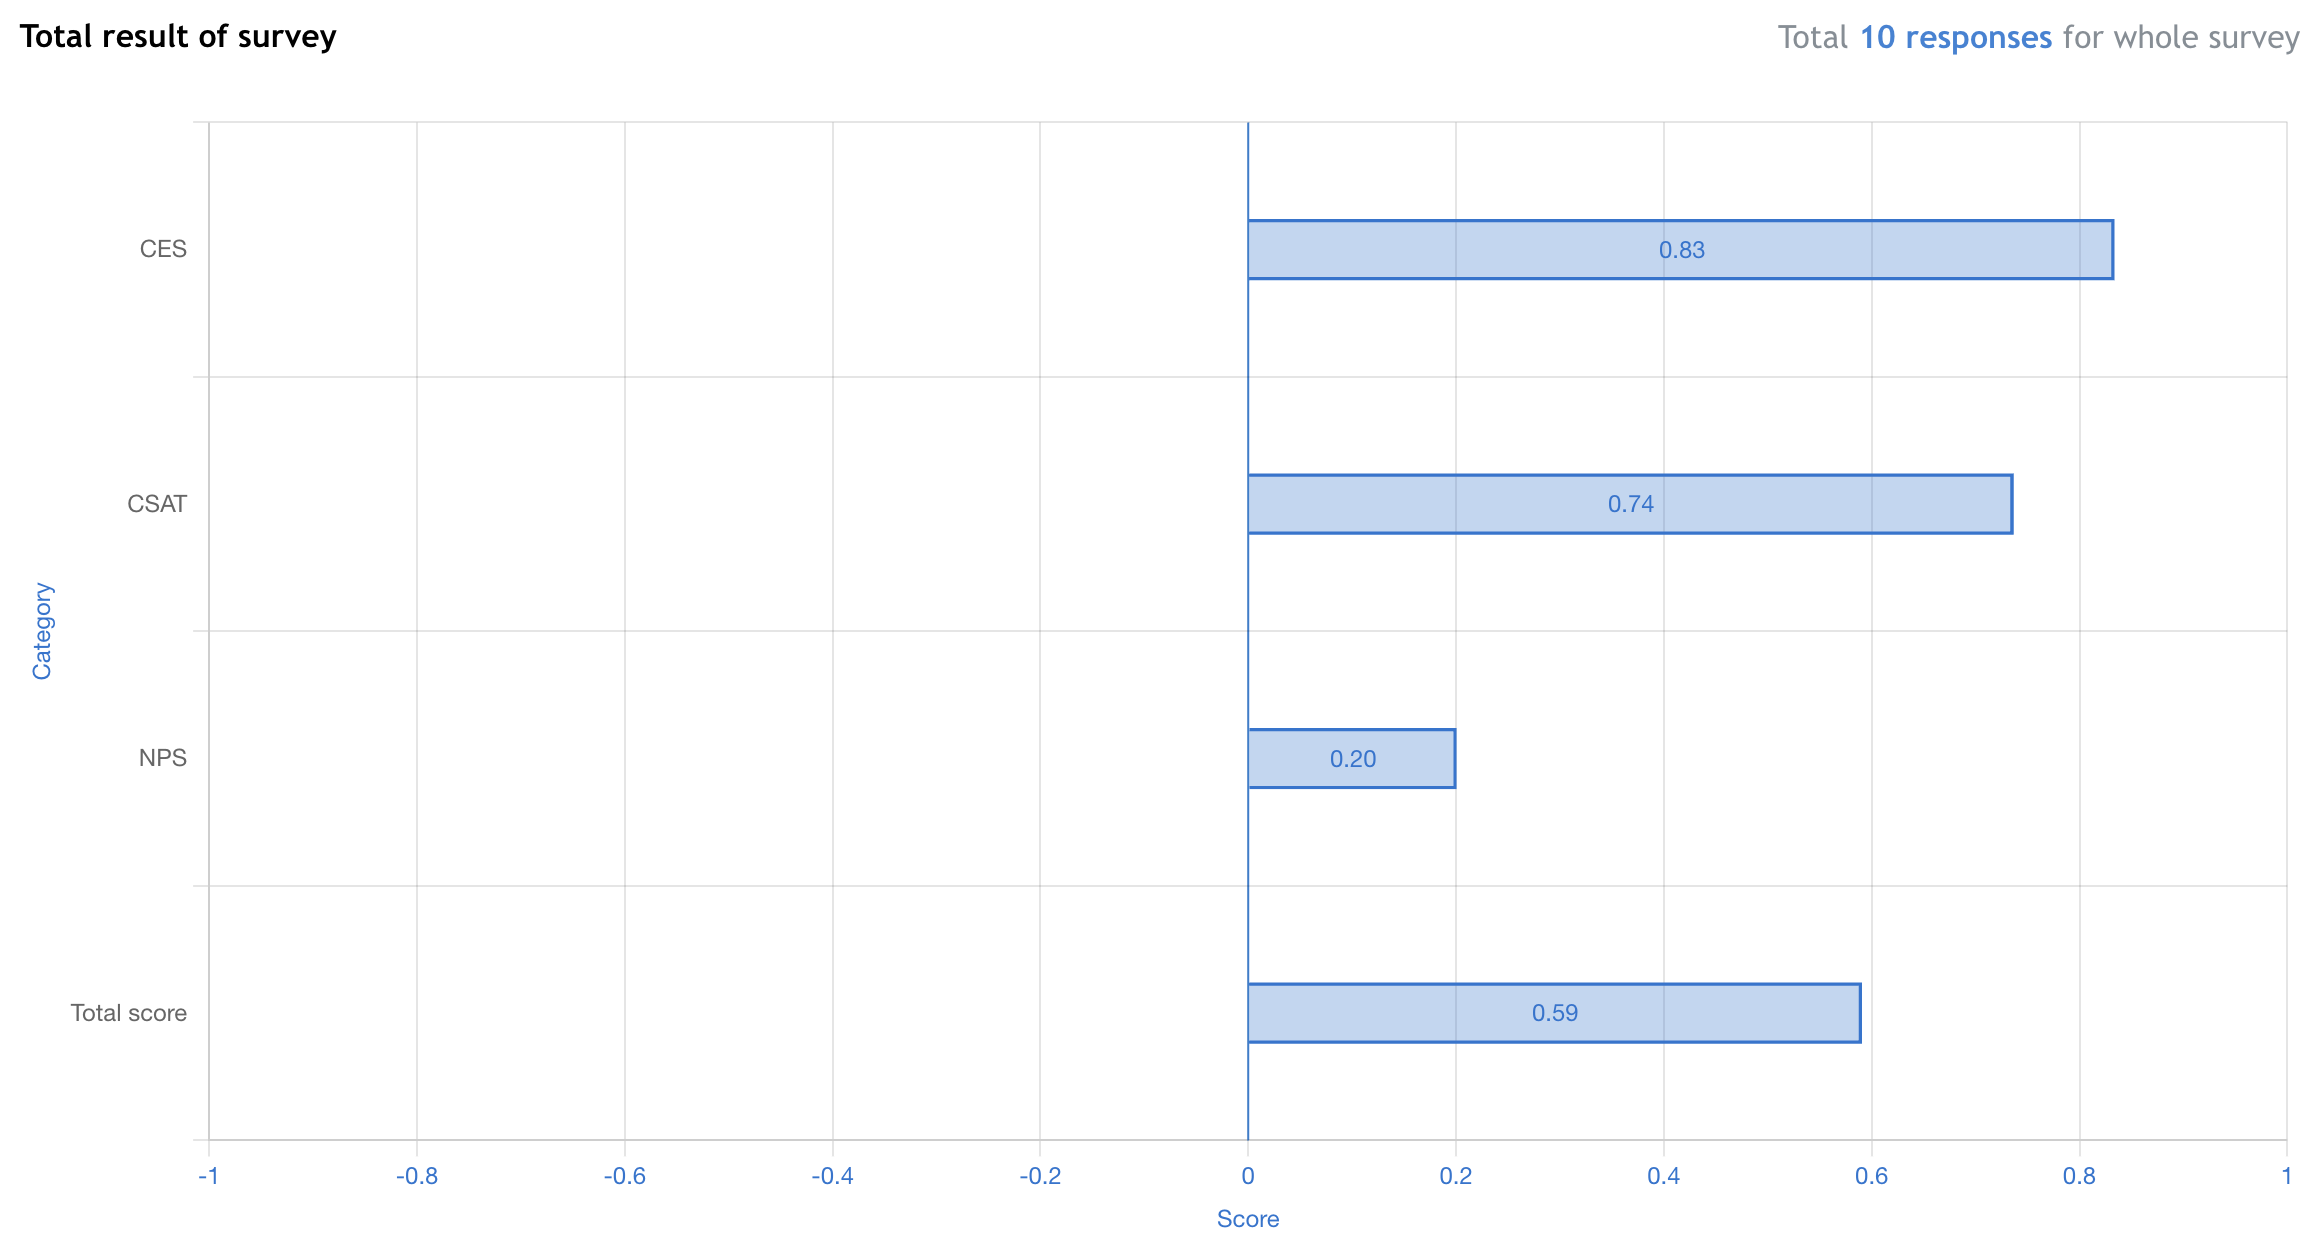
\includegraphics[ width = 0.7\linewidth]{Content/Kiểm thử và đánh giá hệ thống/images/surveyResult2.png}
        \vspace{0.5cm}
        \caption{Kết quả bài khảo sát cho quy trình đổi vé máy bay}
        \label{fig:Kết quả bài khảo sát cho quy trình đổi vé máy bay}
    \end{figure}
\end{center}
Từ kết quả trên, ta thấy rằng kết quả của hệ thống và kết quả tính toán bằng tay khá giống nhau, với điểm số của hệ thống là 0.59, và điểm số tính bằng tay của bài khảo sát là 0.59.
Điểm tổng bài khảo sát cũng là giá trị External Quality của quy trình nghiệp vụ. Giả sử 2 loại quality đều có trọng số như nhau, ta có giá trị trung bình của độ đo 
chất lượng của quy trình nghiệp vụ: 0.645.
\begin{center}
    \begin{figure}[H]
        \centering
        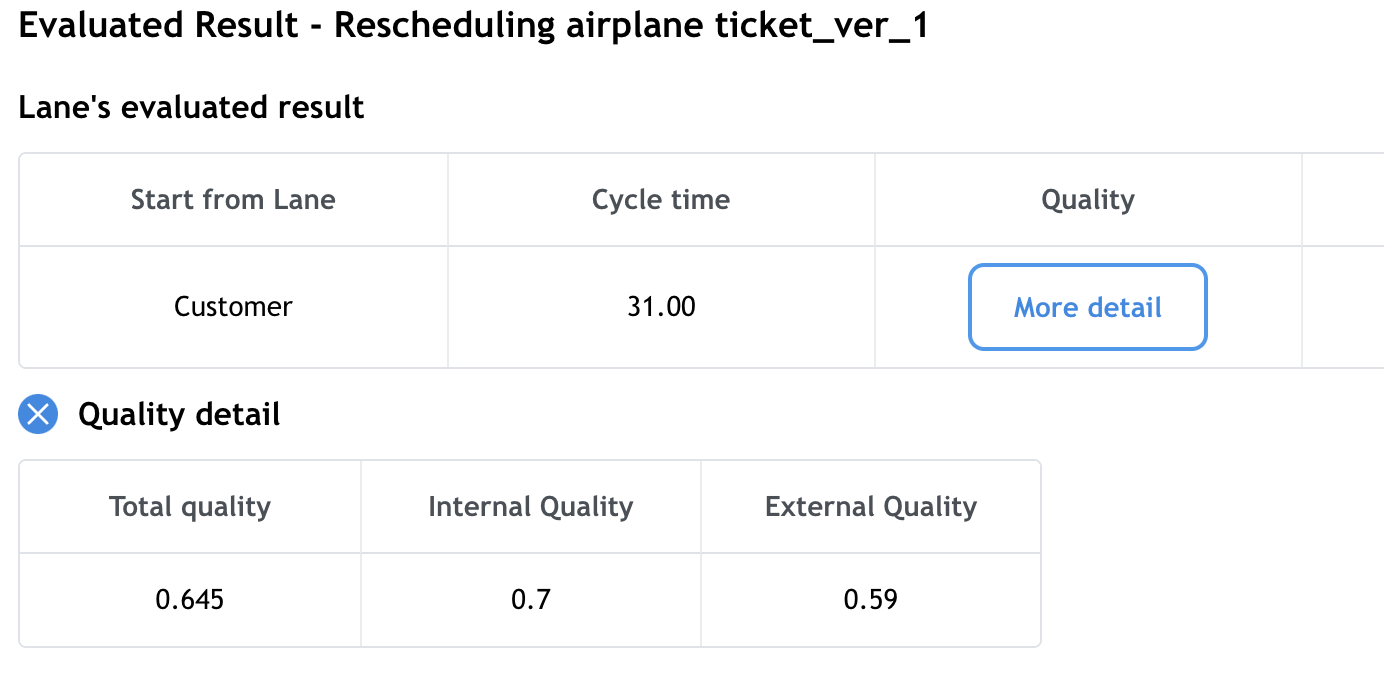
\includegraphics[ width = 0.7\linewidth]{Content/Kiểm thử và đánh giá hệ thống/images/quality2.png}
        \vspace{0.5cm}
        \caption{Kết quả đánh giá chất lượng của quy trình đổi vé máy bay}
        \label{fig:Kết quả đánh giá chất lượng của quy trình đổi vé máy bay}
    \end{figure}
\end{center}
Như vậy, ta thấy rằng kết quả đánh giá chất lượng của hệ thống và kết quả tính toán bằng tay khá giống nhau, với điểm số của hệ thống là 0.645, và điểm số của tính toán bằng tay là 0.645.
    
\subsection{Kiểm chứng process portfolio}
Để tạo ra được process portfolio cho các quy trình nghiệp vụ đang hoạt động trong Workspace, ta cần một số những dữ liệu sau:
\begin{enumerate}
    \item Các giá trị mục tiêu, tệ nhất của các độ đo của Workspace, bao gồm targeted cycle time, worst cycle time, targeted cost, worst cost, 
    targeted quality, worst quality, targeted flexibility, worst flexibility, giá trị của các độ đo feasibility, strategic importance
    \item Các giá trị thực tế của các yếu tố trong độ đo health, bao gồm cycle time, cost, quality, flexibility.
\end{enumerate}

\begin{center}
    \begin{table}[H]
        \centering
        \begin{tabular}{|l|c|}
        \hline
        \multicolumn{1}{|c|}{\textbf{Yếu tố khảo sát}} & \textbf{Giá trị} \\ \hline
        \textbf{Targeted cycle time} & 25 \\ \hline
        \textbf{Worst cycle time} & 50 \\ \hline
        \textbf{Targeted cost} & 20 \\ \hline
        \textbf{Worst cost} & 30 \\ \hline
        \textbf{Targeted quality} & 0.8 \\ \hline
        \textbf{Worst quality} & 0.4 \\ \hline
        \textbf{Targeted Flexibility} & 0.95 \\ \hline
        \textbf{Worst Flexibility} & 0.65 \\ \hline
        \textbf{Feasibility} & 0.8 \\ \hline
        \textbf{Strategic Importance} & 0.7 \\ \hline
        \textbf{Current cycle time} & 30.5 \\ \hline
        Current cost & 28 \\ \hline
        Current quality & 0.7 \\ \hline
        Current flexibility & 0.7 \\ \hline
        \end{tabular}
        \vspace{0.5cm}
        \caption{Bảng giá trị kiểm chứng của các yếu tố trong process portfolio}
        \end{table}
\end{center}

Vận dụng cơ sở lý thuyết được trình bày ở trên, ta tính được các độ đo của quy trình nghiệp vụ để xây dựng process portfolio:
Health = -0.19, Feasibility = 0.8, Strategic Importance = 0.7.
\begin{center}
    \begin{figure}[H]
        \centering
        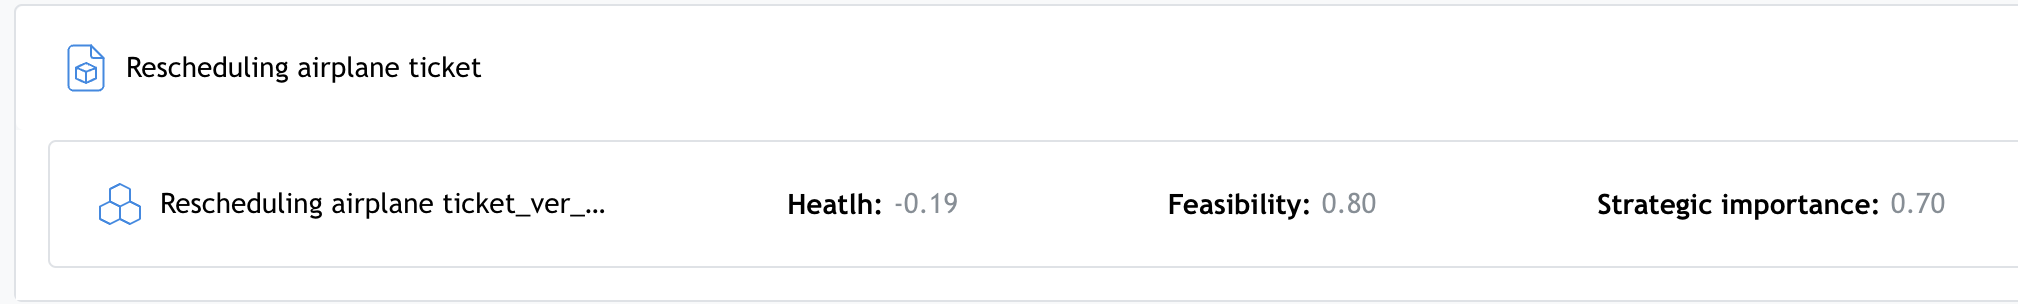
\includegraphics[ width = 0.7\linewidth]{Content/Kiểm thử và đánh giá hệ thống/images/health.png}
        \vspace{0.5cm}
        \caption{Kết quả đánh giá process portfolio của Workspace}
        \label{fig:Kết quả kiểm chứng process portfolio của Workspace}
    \end{figure}
\end{center}
Như vậy, ta thấy rằng kết quả đánh giá process portfolio của hệ thống và kết quả tính toán bằng tay khá giống nhau, với điểm số của hệ thống là -0.19, và điểm số của tính toán bằng tay là -0.19.
Với những kết quả trên, ta có thể kết luận rằng hệ thống đánh giá chất lượng của quy trình nghiệp vụ và process portfolio của Workspace hoạt động hiệu quả và chính xác.